\documentclass[preprint,11pt,review,authoryear]{elsarticle}

\usepackage{graphicx}
\usepackage{caption}
\usepackage{hyperref}
\usepackage{titling}
\usepackage{setspace}
\usepackage{fancyhdr}
\usepackage[headheight=15pt]{geometry}
\usepackage{tikz}
\usepackage{xcolor}
\usepackage{mathptmx}
\usepackage{ragged2e}
\usepackage[pages=all]{background}
\usepackage{docmute}
\usepackage{pdflscape}
\usepackage{longtable}
\usepackage{array}
\usepackage{pdfpages}
\usepackage{lettrine}
\usepackage{tabularx, booktabs}
\usepackage{svg}
\usepackage{silence}
\WarningFilter{natbib}{Citation}

\usetikzlibrary{calc, arrows.meta,shapes.geometric,positioning,shadows.blur,trees}

\title{STU-Jamie_Pinnington_Individual_Project_40 Document}
\author{Jamie Pinnington}
\date{October 28, 2023}

\geometry{
    a4paper,
    total={170mm,257mm},
    left=20mm,
    top=20mm,
}

\definecolor{Border}{RGB}{72, 36, 107} % Border line colour

\backgroundsetup{% Add this block
scale=1,
color=black,
opacity=1,
angle=0,
contents={%

\begin{tikzpicture}[remember picture,overlay]
\draw[line width=2pt, Border] ($(current page.north west)+(1cm,-1cm)$) rectangle ($(current page.south east)+(-1cm,1cm)$);
\end{tikzpicture}% Add 'background lines'
}
}

\fancypagestyle{customStyle}{%
    \fancyhf{}  % Clear all header and footer fields
    \fancyhead[R]{\thepage}  % Place the page number in the top right
    \renewcommand{\headrulewidth}{0pt}  % Remove the header rule
    \setlength{\headheight}{14.49998pt}
}

\begin{document}

\pagestyle{customStyle} % Apply the custom style to all pages

% titlePage
\begin{titlepage} % title page
    
\begin{tikzpicture}[remember picture,overlay]
        \draw[line width=2pt, Border] ($(current page.north west)+(1cm,-1cm)$) rectangle ($(current page.south east)+(-1cm,1cm)$);
    \end{tikzpicture}
    \begin{flushright}
        \vspace*{0.1cm}
        \begin{tabular}{@{}p{6cm}@{}}
            {\fontfamily{ptm}\selectfont \small\textbf{FAO \textit{Dr. Amina Souag, Dr. Hannan Azhar}} \par}
        \end{tabular}
    \end{flushright}
    \begin{center}
        {\fontfamily{ptm}\selectfont \textbf{???????} \par}
        \vspace{0.25cm}
        {\fontfamily{ptm}\selectfont \textbf{BSc (Hons.) Computer Science}\par}
        \vspace{0.25cm}
        {\fontfamily{ptm}\selectfont \textbf{2023-2024}\par}
        \vspace{0.25cm}
        {\fontfamily{ptm}\selectfont \textbf{Individual Project 40}\par}
        \vspace{0.5cm}
        {\fontfamily{ptm}\selectfont \textbf{Title:} \textit{?????}\par}
        \vspace{0.25cm}
        {\fontfamily{ptm}\selectfont \textbf{Author:} \textit{Jamie Pinnington}\par}
        \vspace{0.25cm}
        {\fontfamily{ptm}\selectfont \textbf{Supervisors:} \textit{Dr. Amina Souag, Dr. Hannan Azhar}\par}
        \vspace{0.25cm}
        {\fontfamily{ptm}\selectfont \textbf{Email:} \textit{JP878@canterbury.ac.uk}\par}
        \begin{tabular}{@{}p{12cm}@{}}
            {\fontfamily{ptm}\selectfont This report is submitted in partial fulfilment of the requirement for
            the BSc in \textit{Computer Science} at Canterbury Christ Church University\par}
        \end{tabular}
    \end{center}
    \begin{center}\begin{singlespace}\begin{tabular}{@{}p{15cm}@{}}
                {\fontfamily{ptm}\selectfont I declare that this report is my own original work containing no personal data as defined in
                the Data Protection Act (1998) and that I have read, understood and accept the University's
                regulations on plagiarism/intellectual property rights/research ethics (in particular the
                Research Governance Handbook) and the IP 40 Module Handbook.\par}
            \end{tabular}\end{singlespace}\end{center}
    \begin{center}\begin{singlespace}\begin{tabular}{@{}p{15cm}@{}}
                {\fontfamily{ptm}\selectfont \textcolor{red}{Further, I accept that digital and/or hard copies of my Individual Project 40, or parts thereof, may be made
                    available to other students, individuals and organisations after it has been marked.}\par}
            \end{tabular}\end{singlespace}\end{center}
    \begin{center}\begin{singlespace}\begin{tabular}{@{}p{15cm}@{}}
                {\fontfamily{ptm}\selectfont \textcolor{red}{Finally, I accept that no copy of my Individual Project 40 will ever be returned regardless of the circumstances.}\par}
            \end{tabular}\end{singlespace}\end{center}
    \begin{center}
        {\fontfamily{ptm}\selectfont Signed \textit{Jamie Pinnington}\par}
        \vspace{0.25cm}
        {\fontfamily{ptm}\selectfont Date of Submission: \textit{??????}\par}
    \end{center}
    % Bottom of the page
\end{titlepage}

\clearpage % page 1

\begin{abstract}
\end{abstract}

\section{Acknowledgements}

We'd like to thank the Kaggle community for their invaluable insight and contributions for data augmentations.

\clearpage % page 2

\tableofcontents
\clearpage % page 3

\listoffigures
\clearpage % page 4

\listoftables
\clearpage % page 5

\section{Introduction:}

\lettrine[lines=2]{T}{his} Individual Project documents the conceptualization and development of a machine learning model for translating American Sign Language (ASL) fingerspelling videos into text. The foremost aim of the project, part A, is to create a model that can interpret ASL fingerspelling video and predict the corresponding text to a realistic degree. Given the success of part A, a smaller secondary objective part B is to develop a user-friendly application that allows the user to input ASL fingerspelling videos and receive the corresponding text output. The project outcomes are two-fold, a machine learning model and a user-friendly proof-of-concept that serves academia.

The field of AI has seen rapid development in image and video recognition, however, the most prominently researched topics related to fingerspelling is automatic-speech-recognition (ASR). Interpreting sign language, gestures, and fingerspelling are even smaller niches, and development in these areas is lower. Leading figures such as Bowen Shi \citep{shiFingerspellingDetectionAmerican2021} provided the first attempts to recognize fingerspelling in "wild" environments.

Research for ASL fingerspelling recognition is lacklustre because of its niche topic, and small amount of overall ASL users worldwide, perhaps as high as 2 million \citep{mitchellHowManyPeople2006, ethnologueAmericanSignLanguage2023}. 

Furthermore, the complexity of ASL fingerspelling recognition which has a high degree of variability in hand shape, movement, and speed of signing, and much more characteristics makes recognition a challenging task. This requires a large dataset and a robust model to solve this task, and over the years created datasets are small, lack diversity, and are not developed realistically to a real-world environments.

The purpose of this project is to make use of emerging technologies and datasets in order to produce a model that can further the academic field, and improve accessibility for Deaf and Hard of Hearing individuals. The idea is that for a lot of users fingerspelling is faster than typing on a keyboard or smartphone, and so could provide a means of alternative smoother communication between Deaf and Hard of Hearing individuals, and technology. The model produced in this project will be a proof-of-concept, and will not be a final product, but will serve as a stepping stone for future research and development in the field. 

The Cross-Industry Standard Process for Data Mining \citep{hotzWhatCRISPDM2018}, is a widely used methodology for data mining and artificial intelligence projects. It involves 6 steps that in practice are iterative, and can be revisited at any time as needed. The steps are Business Understanding, Data Understanding, Data Preparation, Modelling, Evaluation, and Deployment.

Over the course of this document, we will document a literature review to discover our roots, following with the CRISP-DM methodology outlining our strategic and technical decisions. In here, expect to find a detailed explanation of the project's development, the model's architecture, and the application's design. We will also discuss the project's management, risks involves, milestones achieved, and state the achieved outcome of the project.

% MAIN CHAPTERS

\section{Chapter 1: Background and Related Work}

The literature review for this project is maintained as a separate piece of work, and so may have repetition to other chapters of this project.
\section{Introduction}
\subsection{Background}
\begin{itemize}
    \item why is this topic (ASL) important? (e.g., accessibility, communication)

    \item what is the specific problem being addressed? (e.g., fingerspelling recognition) (bridges the gap in communication and enhances the learning/usage of ASL.) (makes ai more accessible to this audience?)
          ASL ,
    \item what is the impact of an AI recognizer for this problem? (e.g., enables real-time communication, improves accessibility, etc.) (can this effect broader technology?)
\end{itemize}

Sign language is the primary form of communication for the deaf and hard of hearing community. It allows communication when the spoken language is not possible, and or when the speaker or receiver is deaf or hard of hearing.
Depending on the situation, and like any language, it requires both parties to be fluent in the language to communicate effectively. However, this is not always the case. American Sign Language(ASL) is a complete, complex language that employs signs made with the hands and other movements, including facial expressions and postures of the body, and is used natively in the
United States of America and globally by many individuals. Whilst no attempt has officially been made to survey the language, and most current estimates are based off of historical surveys that prove to be inaccurate\cite{mitchellHowManyPeople2006}. It is estimated that there are over 1 million signers\cite{AmericanSignLanguage}, but others estimates are as high as 2 million\cite{mitchellHowManyPeople2006}.
ASL communicates through a variety of means including gestures, non-manual markers and lexical signs. The most understood are lexical vocabulary, each corresponding to a word or morpheme. Gestures and non-manual markers such as facial expression can complement and convey more interactive or meaningful lexical signs. Additional constructs include usage of space, role shifting and classifiers.

\subsection{Purpose}

\begin{itemize}
    \item what is the purpose of the review?
    \item (e.g., to identify the state of the art in ASL fingerspelling recognition)
    \item (to identify the challenges and opportunities in ASL fingerspelling recognition)
    \item (to identify the most promising techniques for ASL fingerspelling recognition)
    \item * primary purpose is to build our own model, but we need to know what's out there first. *

\end{itemize}
\subsection{Scope}
\begin{itemize}
    \item what is the scope of the review? (e.g., ASL fingerspelling recognition) (what is the scope of the problem? (e.g., real-time recognition of fingerspelling gestures) (what is the scope of the solution? (e.g., image-based recognition of fingerspelling gestures) (what is the scope of the evaluation? (e.g., accuracy, speed, etc.)
    \item what is the scope of the literature? (e.g., papers published in the last 5 years) (what is the scope of the sources? (e.g., peer-reviewed journal articles, conference papers, etc.)
    \item what we're not covering.
    \item only recognition and translation of ASL *fingerspelling* (not full ASL).
    \item specific the application/methodology (e.g., video-based recognition of fingerspelling gestures) (live/stream???)
\end{itemize}

\subsection{Research Questions}
\begin{itemize}
    \item RQ-1: Comparative Analysis of Machine Learning Models:
          What are the strengths and weaknesses of different machine learning models, such as Convolutional Neural Networks (CNNs), Recurrent Neural Networks (RNNs), and Transformer models, in the context of ASL fingerspelling recognition?
    \item RQ-2: Performance Evaluation:
          How do various machine learning models perform in terms of accuracy, processing speed, and reliability for ASL fingerspelling recognition under different conditions (e.g., varying lighting, hand positions, backgrounds)?
    \item RQ-3: Dataset and Model Suitability:
          How does the choice of dataset, including its size, diversity, and quality, influence the effectiveness of different machine learning models in recognizing ASL fingerspelling?
    \item RQ-4: Real-World Applications:
          Considering practical applications like kiosk systems, which machine learning models offer the best balance between technical performance and user experience for ASL fingerspelling recognition?
    \item RQ-5: Technical Challenges:
          What technical challenges are commonly faced across different machine learning models in ASL fingerspelling recognition, and how adaptable are these models to address such challenges?
    \item RQ-6: Impact of Environment Variables:
          To what extent do environmental variables (like hand orientation, motion speed, and background noise) affect the performance of different machine learning models in ASL fingerspelling recognition?
    \item RQ-7: State of the Art and future directions:
          What are the most recent and influential works in the field of ASL fingerspelling recognition, and what are the emerging trends and future directions?
\end{itemize}

\section{Methodology}

\subsection{Literature Identification}
This literature search was completed using the databases IEEE Xplore, Google Scholar, ACM Digital Library, and ScienceDirect. Search terms such as "ASL fingerspelling recognition", "Deep learning for ASL recognition",  "ASL recognition with CNN", "Accuracy of ASL recognition models", "Latest trends in ASL recognition", and "ASL recognition in real-time" were used alone and in conjunction with boolean operators "AND", "OR" to refine the search results. The search was limited to papers published in the last 5 years, and only peer-reviewed journal articles, conference papers, and high quality theses were considered. The search was also limited to papers written in English. The search was conducted in November 2023, and the results were filtered to include only papers that were published between 2018 and 2023.
\subsection{Literature Evaluation}
Of the literature that fit out search criteria, we selected the most relevant papers based on the following criteria: the relevance to the research questions, papers that specifically address ASL fingerspelling, machine learning models in sign language interpretation, papers that used widely recognized datasets relevant to ASL recognition, we chose to exclude editorials, opinion pieces, and non-peer reviewed articles. Papers also required a clear methodology, defined objectives and robust data analysis. Papers with high citation counts were also given preference.
\paragraph{Organizing and Categorizing}
This subsection describes how the selected literature was organized and categorized, providing the basis for a comprehensive synthesis.

\paragraph{Comparative Analysis}
A detailed comparative analysis of the methodologies and findings of the selected studies is presented here, highlighting similarities and differences in approaches.

\paragraph{Gaps and Trends}
This part identifies any gaps in the current research landscape and notes emerging trends in ASL fingerspelling recognition technology.

\paragraph{Conclusions and Narrative}
The conclusions drawn from the comparative analysis and their relation to the original research questions are discussed here, forming a narrative that captures the current state of the field.

\paragraph{Visual Representation and Critical Evaluation}

\begin{landscape}
    % !TeX root = main.tex
\newcolumntype{L}{>{\raggedright\arraybackslash}p{0.195\textwidth}}

\begin{footnotesize}
    \begin{longtable}{LLLLLLL} % Adjust the column width as needed
        \caption{Summary and Analysis of ASL Fingerspelling Recognition Models (2018-2023)}
        \label{table:asl-comparison}                                                                                                                                                                                                                                                                                                                                                                                                                                                                                                                                                                                                          \\
        \toprule
        Reference                                          & Model Used                                                                                                            & Framework                & Dataset                        & Key Findings                                                                                                                                              & Performance Metrics                                    & Challenges Addressed                                                                                                                                                    \\
        \midrule
        \endfirsthead
        \toprule
        Reference                                          & Model Used                                                                                                            & Framework                & Dataset                        & Key Findings                                                                                                                                              & Performance Metrics                                    & Challenges Addressed                                                                                                                                                    \\
        \midrule
        \endhead
        \bottomrule
        \endfoot
        \endlastfoot
        \cite{skumarTimeSeriesNeural2018}                  & RNN, LSTM, Attention, Encoder/Decoder                                                                                 & [Not Specified]          & NCSLGR Corpus                  & Recognition and translation of ASL glosses                                                                                                                & GRR: 86\%, GER: 23\%                                   & Real-time recognition and translation                                                                                                                                   \\

        \cite{weerasooriyaSinhalaFingerspellingSign2022}   & RF, KNN, LR                                                                                                           & [Not specified]          & FASSL custom dataset           & Developed a classifier for static signs using a small dataset                                                                                             & Accuracy: 87.9\% (correct estimates)                   & Pose classification with limited data                                                                                                                                   \\

        \cite{cihancamgozSignLanguageTransformers2020}     & Transformers with CTC loss                                                                                            & PyTorch                  & PHOENIX14T                     & State-of-the-art results in recognition and translation                                                                                                   & WER, BLEU-4 scores                                     & Translation from sign language videos to spoken language sentences                                                                                                      \\

        \cite{abiyevReconstructionConvolutionalNeural2020} & CNN, SSD, FCN                                                                                                         & [Not specified]          & Kaggle ASL Fingerspelling      & High accuracy, vision-based translation                                                                                                                   & Accuracy: 92.21\%                                      & Real-time translation, robustness in ASL recognition                                                                                                                    \\

        \cite{bantupalliAmericanSignLanguage2018}          & CNN, LSTM, RNN                                                                                                        & OpenCV                   & Self-created Dataset           & Effective recognition with custom CNN model                                                                                                               & Accuracy: 98.11\%                                      & Robust recognition in controlled environments                                                                                                                           \\

        \cite{kabadeAmericanSignLanguage2023}              & ResNet, Bi-LSTM, CTC, Attention                                                                                       & [Not specified]          & ChicagoFSWild                  & Recognition using optical flow and attention, preprocessing for occlusions                                                                                & Letter accuracy: 57\%                                  & Recognition in 'wild' conditions, occlusions                                                                                                                            \\

        \cite{shiAmericanSignLanguage2018}                 & CNN, LSTM, CTC                                                                                                        & Faster R-CNN             & Custom YouTube Dataset         & Improved accuracy with hand detection                                                                                                                     & Test Acc: 41.9\% with CTC                              & Recognition in the wild, varying conditions                                                                                                                             \\

        \cite{shiFingerspellingRecognitionWild2019}        & CNN, RNN, CTC, Attention                                                                                              & TensorFlow               & ChicagoFSWild, ChicagoFSWild+  & Enhanced recognition in uncontrolled environments                                                                                                         & Word Error Rate: 27.2                                  & Recognition in diverse and challenging real-world scenarios                                                                                                             \\

        \cite{shiFingerspellingDetectionAmerican2021}      & 2D/3D-CNN, Bi-LSTM                                                                                                    & OpenPose                 & ChicagoFSWild, ChicagoFSWild+  & Superior detection in uncontrolled environments                                                                                                           & AP@IoU: 0.495, MSA: 0.386                              & Handling fine-grained handshapes and signer’s pose                                                                                                                      \\

        \cite{nguyenDeepLearningAmerican2019}              & 1) LBP, HOG descriptors, multi-class SVM, 2) End-to-end CNN 3) CNN weights as feature extractor for Linear-kernel SVM & [Not specified]          & Massey Dataset                 & Three diverse methods for fingerspelling recognition                                                                                                      & Recognition rate: 97.49\%, 98.23\%, 98.30\%            & Adaptability in feature extraction and classification approaches                                                                                                        \\

        \cite{chongAmericanSignLanguage2018}               & SVM and DNN                                                                                                           & TensorFlow, Scikit-learn & Self-created Dataset           & Comparison of SVM and DNN for ASL recognition; effective use of LOO approach for bias avoidance                                                           & Recognition rate: 72.79\%, 88.79\%                     & Multi-class classification with 36 classes (26 letters and 10 digits)                                                                                                   \\

        \cite{bantupalliAmericanSignLanguage2018}          & CNN (Inception) for spatial features, LSTM for temporal features                                                      & TensorFlow, Keras        & American Sign Language Dataset & Efficient extraction of temporal and spatial features; use of Inception and LSTM models                                                                   & Accuracy up to 93\% (Softmax Layer), 58\% (Pool Layer) & Managing longer sequences with LSTM; preventing overfitting with dropout                                                                                                \\

        \cite{shiSearchingFingerspelledContent2022}        & FSS-Net (End-to-End Model for Fingerspelling Detection and Text Matching)                                             & [Not Specified]          & ChicagoFSWild, ChicagoFSWild+  & Introduced explicit temporal localization for fingerspelling search and retrieval. Demonstrated effective fingerspelling detection in varying conditions. & mAP: 0.684 (YouTube), 0.584 (DeafVIDEO), 0.629 (Misc)  & Fingerspelling detection in diverse visual conditions; handling open vocabulary and arbitrary-length queries; confusion between similar handshapes; detection failures. \\

        \cite{gajurelFineGrainedVisualAttention2021}       & Fine-Grained Visual Attention with Transformer Model (CTC, CNN, LSTM)                                                 & [Not specified]          & ChicagoFSWild                  & Significantly improved state-of-the-art performance in fingerspelling recognition using Transformer-based contextual attention mechanism                  & Letter Accuracy: 46.96 \% (dev), 48.36\% (test)        & Addressed challenges in capturing fine-grained details in unsegmented continuous video data. Focused on improving generalization and regularization of the model.       \\

        \bottomrule
    \end{longtable}
\end{footnotesize}
\end{landscape}

\subsection{Report Structure}
- what is the structure of the report? (e.g., introduction, literature review, etc.) (aka roadmap?)

\subsection{Conclude Introduction}

\begin{itemize}
    \item By understanding, the insight gained from this review will be used to inform the design and implementation of our own model.
    \item * evidence based approach is neccessary to be impactful *

\end{itemize}
\section{Historical Context} % RQ-7
\begin{itemize}
    \item Evolution of ASL fingerspelling recognition
    \item Major milestones and breakthroughs
\end{itemize}

\section{Methods and Techniques} % RQ-1, RQ-2, RQ-3
\begin{itemize}
    \item Overview of methods used in the literature
    \item Image/Video-based Approaches
    \item Framework-based Approaches (e.g., MediaPipe)
    \item Hybrid methods
    \item Evaluation metrics commonly used
\end{itemize}

\section{Challenges in ASL Fingerspelling Recognition} % RQ-5, RQ-6
\begin{itemize}
    \item Technical challenges (e.g., diverse handshapes, background noise)
    \item Data challenges (e.g., lack of large labeled datasets)
    \item Real-world challenges (e.g., different lighting conditions, user variability)
\end{itemize}

\section{Overcoming Obstacles} % RQ-5
\begin{itemize}
    \item Techniques to enhance accuracy
    \item Data augmentation strategies
    \item Transfer learning and pre-trained models
\end{itemize}

\section{State of the Art/Real-World Applications} % RQ-4, RQ-7
\begin{itemize}
    \item Most recent and influential works in the field
    \item Comparison of different methods' performance
    \item Real-world applications and success stories
\end{itemize}

\section{Future Directions and Open Challenges} % RQ-7
\begin{itemize}
    \item Emerging trends in the field
    \item Areas that need further research
    \item Potential impact of advancements (e.g., in deep learning)
\end{itemize}

\section{Ethical and Societal Considerations}
\begin{itemize}
    \item Data privacy concerns
    \item Bias and fairness in ASL recognition models
    \item Implications for the deaf and hard of hearing community

\end{itemize}

\section{Main Conclusion}
\begin{itemize}
    \item Summary of the main findings of the review
    \item Reiteration of the importance of the topic
\end{itemize}
\section{Chapter 3: Methodology}

\begin{figure}[h]
    \centering
    \includegraphics[width=0.5\textwidth]{images/CRISP-DM-process-model_W640.jpg}
    \caption{CRISP-DM Methdology \citep{lofstromUtilizingDiversityPerformance2009}}
    \label{fig:CRISP-DM}
\end{figure}

The CRoss Industry Standard Process for Data Mining (CRISP-DM) is a widely used methodology that provides a structured approach to undertaking data science projects from a process perspective. In this task, we emphasize the usage of CRISP-DM methodology as a preferable process over a standalone software development methodology, this is because the project requires a higher level of management than a naive implementation that agile gives. Agile-like processes can be integrated into CRISP-DM with usages of rapid prototyping and usual backlogging, testing, etc, but found the CRISP-DM "pipeline" is adaptable to the real world goal of developing data science projects.

CRISP-DM is inherently iterative, it understands that whilst developing in say the evaluation phase, unexpected consequences allow us to move back to the data preparing or modelling phase to adjust. Furthermore, the feedback loops observed in Figure \ref{fig:CRISP-DM} explicitly accommodates returning to previous steps to refine insights. 

The 6 phases include business understanding, data understanding, data preparation, modelling, evaluation, and deployment.

\subsection{Business Understanding}

The objective of the project is to increase accessibility for the Deaf and Hard of Hearing community, and by developing artificial intelligent models, this would be achieved. In order to tackle this, we must understand if we have the ability to; developing AI requires computing resources (hardware platforms), as well as software, furthermore we must understand if the datasets available exist in order to complete the objectives, and if there are any data security concerns and or legal issues.

The computer resource available to us are NVIDIA RTX 3090 GPU with 24 GB of GDDR6X memory, an AMD Ryzen 9 7950X 16-Core Processor and 64 GB of DDR5 memory. This is critical because one, seq2seq tasks can require a lot of memory and processing power from graphics cards / accelerators due to the amount of parameters and input sizes, and an NVIDIA monopoly due to the CUDA framework \citep{CUDAToolkitFree}.

At this early stage, we must decide upon the major tools. Artificial intelligence splits into two major deep learning frameworks, and are TensorFlow \citep{abadiTensorFlowSystemLargescale2016} and PyTorch \citep{paszkePyTorchImperativeStyle2019}. PyTorch has a tremendous amount of modularity, and out of the box support for major models, comparing memory consumption and speed is harder than implementations of models are different, but is it generally agreed PyTorch is faster and has lower memory consumption.

\begin{figure}[h]
    \centering
    \includegraphics[width=1\textwidth]{images/pytorch-vs-tensorflow-popularity-comparison.png}
    \caption{TensorFlow vs PyTorch \citep{boeschPytorchVsTensorflow2023}}
    \label{fig:tfvspt}
\end{figure}

See Figure \ref{fig:tfvspt}, that shows the number of created repositories, i.e. new projects with certain frameworks. For a comparison on these frameworks from Gardenz Boesch \citep{boeschPytorchVsTensorflow2023} and anecdotal evidence from increasing usage from popular data science website Kaggle \citep{anthonygoldbloomKaggleYourHome}, we conclude on PyTorch due to its ease of use modular system, out-of-box features, and increasing popularity shift compared to TensorFlow.

The "ASL Fingerspelling Recognition Corpus (version 1.0) is a collection of hand and facial landmarks generated by MediaPipe version 0.9.0.1 on videos of phrases, addresses, phone numbers, and urls fingerspelling by over 100 Deaf signers" \citep{asl-fingerspelling} released by Google with a licence to adapt and use freely, even commercially \citep{CCDeedAttribution}. This dataset presents an opportunity, released shortly before this projects conception in early 2023. It is a large dataset in size (180 GB) consisting of diverse conditions, number of signers, representation of signing fluency and cultures, essentially the complexity of the dataset allows a larger and more complicated model as the amount of features that can be extracted is high. This dataset can change the playing field, as previous research for ASL fingerspelling came from the ChicagoWild \citep{fs18slt} and ChicagoWild+ \citep{fs18iccv} datasets, which were the largest ASL fingerspelling collections "in the wild" conditions, essentially videos available online, predominately used by Bowen Shi \citep{shiAmericanSignLanguage2018}. 

Academic research, as well as applied research has been moving away from these datasets due to legal issues regarding the source of the datasets, videos from the public realm such as YouTube were being downloaded and used without permission, this presented legal issues, and thus commerciality of models developed with it impossible would be of heightened concern.


\subsection{Data Understanding}

Given our chosen dataset, we must explore the data we are working with. This includes the complexity of the data, in terms of size, shape, format, distribution, and quality. We need to model the data, so we can understand the relationships between fields. The data was created using MediaPipe \citep{lugaresiMediaPipeFrameworkBuilding2019}, an open-source framework for creating AI pipelines, it contains various pre-trained models that can label images and videos, for groups of the body such as hands, face, and pose.

\begin{figure}[h]
    \centering
    \includegraphics[width=0.75\textwidth]{images/hand-landmarks.png}
    \caption{MediaPipe Framework Hand Landmarks \citep{lugaresiMediaPipeFrameworkBuilding2019}}
    \label{fig:handlandmark1}
\end{figure}

Figure \ref{fig:handlandmark1} shows the mapping of landmarks for hands, which are points used to track the movement of the joints and important features, all groups have this structure. The dataset consists of 121 parquet files, columnar-storage structure for large datasets that work in a distributed environment such as Hadoop

\begin{figure}[h]
    \centering
    \includegraphics[width=0.75\textwidth]{images/parquet_structure_1.png}
    \caption{Dataset Structure: train.csv}
    \label{fig:datastructure1}
\end{figure}

The first figure, referenced as Figure \ref{fig:datastructure1}, illustrates the train.csv file where each sequence\_id corresponds to a signed phrase, linking to a separate document. Each sequence\_id organizes multiple sequences or rows of frames, with the subsequent columns detailing landmarks divided into their x, y, and z coordinates.

\begin{figure}[h]
    \centering
    \includegraphics[width=0.75\textwidth]{images/parquet_structure_2.png}
    \caption{Parquet File Structure}
    \label{fig:datastructure2}
\end{figure}

The second figure, referred to as Figure \ref{fig:datastructure2}, depicts the structure of a Parquet file, highlighting that the dataset is sequential. Analysis of the dataset reveals variability in the length of phrases and the number of frames per sequence. The dataset comprises 1,629 spatial coordinates that capture the x, y, and z positions for each of the 543 landmarks identified across categories like 'face', 'left\_hand', 'pose', and 'right\_hand'.

Exploring the dataset, we create a Python script, and use pip packages such as pandas, pyarrow, and numpy to load and manipulate the data. Pandas and pyarrow allows us to load the parquet into a data frame to get some characteristics of one file.

\begin{figure}[h]
    \centering
    \includegraphics[width=0.65\textwidth]{images/distro_chars.png}
    \caption{Distribution of Phrase Lengths (no. of characters)}
    \label{fig:distro_chars}
\end{figure}

\begin{figure}[h]
    \centering
    \includegraphics[width=0.65\textwidth]{images/distro_frames.png}
    \caption{Distribution of Sequence Lengths (no. of frames)}
    \label{fig:distro_frames}
\end{figure}

The length of the phrases, by the number of characters is at most 32, there are a number of short phrases which would need to be investigated further less than 10. 

The length of sequences is highly variable whereas the phrases is not so much. The length of sequences seems to reflect with the length of phrases but is weighted towards shorter sequences, as the number of frames increases, the number of characters in the phrase increases in order to complete the phrase. Given potential clipping errors, there seems to be outliers from 400+ frames, which might signify a failure by signer to stop the recording, or a failure in the recording process. This makes plausible sense as there are no phrases in that ball pack area. There's an understanding that phrase lengths are not tightly clipped, and unnecessary frames exist at the end, which should correlate to actual fingerspelling.

There are a number of NaN values, for where landmarks have no value, this could be due to the holistic model unable to detect, or the landmark simply wasn't in frame at that time.

\subsection{Data Preparation}

For the code for the data preparation and preprocessing, please refer to \ref{G}. Preparing the dataset is a critical step, and can be as important as the model itself. The 121 parquet files contains the 68 parquet files totalling 95 GiB, each roughly 1.4 GiB, from the training set, and 53 parquet files from a supplemental set. The model we decide to use, will have to loop over the data given in iterations called epochs, each epoch a run through of the data, and the model will learn from the data, and adjust its weights and biases to minimize the loss function. The two parts of the dataset are nominal throughout, so we could only use the training set which reduces the overall size of the dataset to 95 GiB and inputs steps into the model per epoch.

Depending on the model chosen, certain preprocessing can happen at run-time or before the model is trained. The dataset must be prepared, so that it is in a format that most machine learning models can understand. This also includes performing augmentations, which are transformations on the data that should enhance the quality of the data, but do not necessarily change the underlying meaning of it. This is done to increase the robustness of the dataset, so that complex models can extract features without over or under fitting, and by doing so the model can train for longer. At some point data augmentation becomes trial and error.

The parquet files of the dataset are too large to be kept in memory, and the size of the data should be as minimum as possible without losing value. For the preprocessing stage we use TensorFlow's TFRecord file format, which allows us to store large amounts of data in binary format, which reduces the overall disk size used to 19.2 GiB, with the average TFRecord while being reduced over 85\% to 160 MiB. This is advantageous to do because as we require constant tinkering due to the CRISP-DM methodology, we require data that can be preprocessed quickly instead of waiting for this step before training.

Furthermore, this saves our computing resources that could be crucial in allowing us the largest possible model.

There are a number of common data augmentations that are used in image and video processing, such as rotation, scaling, translation, flipping, and cropping, removing, random replacement of tokens, adding artificial noise, and more. 

The file\_id of each parquet file is processed to create a TFRecord file, it is read and the columns of the sequence\_id as well as a selection of columns is extracted. The selection columns are the landmarks for the hands, face, and pose, that we have grouped, and specified the x, y, and z coordinates. We take a large range of the face to include lips and eyes, all the left and right hand, and 23 of the pose, which excludes the forearms.

Standard scaling for the FACE, LHAND, RHAND, POSE is performed with respect with mean and standard deviation to normalize the data so that essentially all landmarks of that group are equally treated so that larger valued features aren't prioritized. This can increase model performance of models with gradient descent optimization and neural networks with non-linear activation functions.

Referring back to Figure \ref{fig:distro_frames} we recall different chunks at frames 256 and 384, we will use these as the maximum frame lengths. The sequences that are above this maximum length we don't want to truncate as the rest of the frames could be important, and we'd lose valuable data compared to its target. Interpolation is used to create a sequence of frames that extrapolates a linear trend from the existing frames beyond the maximum length. This is an attempt to maintain the integrity of the data, but to shorten it.

Next, the unhandled NaN values are filled with 0s as the model will simply not be able to process NaNs. The NaNs, now 0s, are counted for the left and right hand, which are used to create a process whereby we remove corrupted data that is short, and has no hands. Mikel Bober-Irizar found that by using the levenstein distance and greedy decoding, found the average string which is used to fill in \citep{mikelbober-irizarStaticGreedyBaseline}.

Sequences where twice the length of the target phrase is less than the maximum amount of NaNs from the left or right hand are serialized and moved into a schema where a single sequence contains all its landmarks and corresponding frames equating to the target phrase it represents. It is then written to file. The features are stored as a FloatList, and the phrase is stored as a ByteList with utf-8 encoding. 

This whole process is used with Python's multiprocessing library, which allows us to run the process a number of items at once, keeping in sync. This speeds up processing by a factor of the number of processes allocated. Preprocessing that takes 10 minutes with 8 cores takes roughly 1.25 minutes.

\section{Chapter 4: System Design and Architecture}

\subsection{Modelling}

At this point, we have a sufficient pipeline of preprocessing. Given our literature review, there are a multitude of machine learning and deep learning models. Transformers are still state-of-the-art in seq2seq tasks, and our choice of PyTorch as a framework we must perform our preprocessing steps that will occur at runtime.

A Transformer in PyTorch has an expectation that the shape of the data at the input is [batch size, sequence length, features]. The batch size is the number of sequences that are inputted at once, the sequence length is the number of frames in the sequence, and the features are the number of landmarks. PyTorch has a system whereby data pipes are used to modularly create a stream of data, this can be used to create a data loader that can be used to feed the model, this can be done in parallel with other processes to increase input.

Referring to \ref{F}, specifically \ref{fig:pp_runtime} for a large overview of the pre-processing that is completed to serve the Transformer as well as \ref{G} for the implementation.

The usage of data pipes allows us to iteratively stack pipes, and perform transformations on the data, the newly created TFRecords are split 80:20 for the train and validation set. The config of the pipe is used to slice TFRecords depending on where we want the index to start and end, take a training set which would be 0-96 for the full set.  A shuffler is used to list and buffer TFRecords into memory, the iterable pipe then opens the file in binary mode, opens and decompressed the file, loading an Example. 

Previously, during the creation of the TFRecords, we encapsulated the features and phrases of the dataset into a structure known as an Example. Each Example is a serialized representation of a single data instance, and in our setup, it was defined to include a sequence of landmarks, frames, and a target phrase. Once deserialized, these records are processed through tokenization. Tokenization can vary, from ordinal to one-hot encoding, but it essentially involves converting the characters of the phrases into numerical formats. For use with a Transformer model, this conversion generates a list of tensors. Additionally, we prepend a start token at the beginning of each sequence and append an end token at the end to facilitate processing. The tokens are important for the model to understand the beginning and end of a sequence, and to differentiate between the two. A model should learn when to start and stop predicting additional tokens.

Transformers are designed to handle variable-length sequences by padding them to a uniform length within each batch. This is why the maximum sequence length was previously set to either 256 or 384. With a batch size of 128, both the sequence frames and the tokenized phrases are padded with specific tokens to reach this maximum length. For the sequence frames, a padding token of 0 is used, and for the tokenized phrases, a special class token indexed as 61 is used, ensuring all sequences within a batch are of the same length.

At the same time, we calculate and pass on a list of the original lengths of the sequences frames  and target phrase before padding.

For an in-depth explanation of Transformers, refer to \cite{vaswaniAttentionAllYou2023}. Other than changing the parameters to fit the dimensionality and task of our dataset, the original Transformer uses positional encoding to give the model information about the order and position of tokens in a sequence. We employ learned positional embeddings instead, which are trained alongside the model. This allows the model to learn a more optimal, specific positional encoding for this task.

Our model has an encoder and a decoder, it has 8 encoder layers, 2 decoder layers, and 4 heads each. The input is passed through an 3 1d convolutional layers to extract features, and concatenated with an embedding layer, and passed through the encoder. The target tokens are passed through an embedding layer to generate token embeddings, and are concatenated with another embedding layer. This gives the tokens positional information which should provide more nuanced relationships.

The lengths of the source and phrases that we retained earlier, are used to mask the inputs to the model. Transformer will attend to all tokens, but we want the model to not attend to padding tokens, as well as being able to cheat and lookahead. We provide padding masks that apply 0s to the padding tokens, and the Transformer doesn't attend to these tokens are the score is minimal. We also provide a look-ahead mask for the target, which is a triangular matrix that masks the future tokens. These are critical for the model to learn that it is decoding, and not classifying, as the model should only be predicted the next token given the previous.

There were a number of additional steps that were used to modify the model, such as label smoothing, which is a regularization technique that prevents the model from becoming too confident in its predictions. We also experimented with increased dropout, and weight decay of the optimizer. We used a fused AdamW optimizer, an optimizer is controller that updates the weights and biases of the parameters in the model per step or batch given the returned loss function. AdamW was used with a stacked learning rate scheduler, that gave a warm-up period of 10 epochs followed by 190 epochs with CosineDecay scheduler, a scheduler is a function that changes the learning rate of the optimizer slowly over time. This allows the gradients and parameters to "warm up" and then slowly converge to a minimum, this is important as the model can get stuck in local minima, and not converge to a global minimum.

After hand rolling everything we moved to a library called PyTorch Lightning. After hundreds and hundreds of lines of PyTorch code, Lightning \citep{williamfalconWelcomePyTorchLightning} greatly reduces boilerplate, has a lot of optimization and allows you to focus on what's important. We were able to change the precision of our model from 32-bit to bf16-mixed, which is a mixed precision training that uses 16-bit floating point numbers for the model weights and 32-bit for the gradients. This reduces the memory usage and speeds up training, by almost 2x.

A lot of manual work is moved into simple Lightning modules which are wrappers around your model architecture, it also has a data module to encompass the data pipeline, and a trainer to control the training, validation and prediction loops. This allows us to greatly enhance the ease of use of PyTorch natively.

In this stage, we were constantly iterating to find something that was good enough to move in that direction with.

\newpage 
\section{Chapter 6: Testing and Validation}

\subsection{Evaluation}

During the early stages of development, the model was evaluated using Ray Tune \citep{RayTrainScalable}. Initially, due to simpler model architectures and lower memory requirements, it was feasible to concurrently run multiple instances (typically 2 or 4) to test various hyperparameters. These parameters included batch size, gradient accumulation, learning rates, feature dimensionality, the number of heads and layers, sequence length, type of optimizer, fusion techniques, and schedulers. This comprehensive testing was crucial to understand how different configurations influenced the model's performance on the dataset.

As the training progresses, the model utilizes the CrossEntropy loss function to gauge the discrepancy between the predicted probabilities and the actual target labels across 62 classes. Each training step involves generating a probability for the next token, with the loss being calculated as the negative logarithm of the probability assigned to the correct token, summed across all predictions. Following the loss calculation, the model undergoes back propagation—adjusting its weights and biases to minimize the loss. This optimization is repeated iteratively with each batch. Ideally, this should result in a reduction of training loss over time. Simultaneously, it is expected that the validation loss should decrease at a comparable or better rate, contingent on the level of regularization applied.

Referring to Figure \ref{fig:trainvsval} substantial regularization, such as L1/L2 and dropout, intentionally impairs the training performance by temporarily disabling numerous neurons within the Transformer's feed-forward network. This approach, while potentially increasing training loss, enhances the model's ability to generalize to unseen data. This explains why the training loss may occasionally exceed the validation loss. This allows the model training to remain on the rails for longer.


\begin{table}[htbp]
    \centering
    \caption{Edit Distance Comparison}
    \begin{tabular}{lll}
        \toprule
        Predicted                                & Target                                   & Edit Distance \\
        \midrule
        + wust tannot figure this out            & i just cannot figure this out            & 3.0           \\
        +t r ahoulders anees and toes            & head shoulders knees and toes            & 6.0           \\
        +he ftn of the parts                     & the sum of the parts                     & 4.0           \\
        +o nou gike to go camping                & do you like to go camping                & 3.0           \\
        +aare ts a high priorita                 & space is a high priority                 & 5.0           \\
        +o n good deed to some                   & do a good deed to someone                & 5.0           \\
        + good stimulus deserves a bood response & a good stimulus deserves a good response & 2.0           \\
        +ou aall aose your aoice                 & you will lose your voice                 & 5.0           \\
        +ware did you get tuch a silly idea      & where did you get such a silly idea      & 4.0           \\
        
        \bottomrule
    \end{tabular}
    \label{tab:edit_distance}
\end{table}

After inference of 5137 targets, we logged the predicted string, target string, and the edit distance. The model quite quickly understood what the end token was, and so we eventually assigned most if not all padding tokens as end tokens. For inference, we sliced the string from the first end token, to the target without the start token and end token. This was used to calculate the mean levenstein distance, of which was 4.7, and with a mean length of 28.7 for the target phrase. This gives us an error rate of 16.37\%.

We used Lightning to perform inference using the predict step, which was used on a holdout set, which was a set of data that the model had never seen before. The Levenshtein or edit distance, is the minimum number of single-character edits required to change one word into another. This was used to calculate the distance between the predicted phrase and the target phrase. The edit distance was calculated for each phrase in the holdout set, and the average was taken. The lower the edit distance, the better the model is at predicting the target phrase. \ref{tab:edit_distance} shows a selection of the predicted phrases, the target phrases, and the edit distance between them. It seems we have a bug in our code, the predicted phrase starts on the first character, but it doesn't seem to make a prediction despite having an input yet. However, it is still quite robust at long and short phrases, and is definitely readable.



\section{Chapter 7: Management of Project}

In regard to the project management, CRISP-DM invaluable in setting out how to begin and in what steps, which was preferred over a software development methodology alone. The project was managed using a Gantt chart \ref{fig:GanttChart}, which was used to plan and track the project's progress. It worked very well up until March, the project was on track, and our risk register \ref{fig:Risk Register} included a high potential risk of overflowing project time due to project complexity. Project halted for a whole month as the model was not performing as expected, and so the project was behind schedule. The project was able to recover, this was possible down to streamlining the development process by bringing in Ray Tuning and Lightning. This allowed the model to be training multiple hyperparameters at all times.

The usage of work break down documents such as \ref{fig:WBS: Build Application} were more prominent early on, they allowed us to set expectations of the work that was required and to move in a structured way. As we moved deeper into the model development in regard to augmentations, these became less useful as the work was more iterative.

\section{Ethical Considerations Chapter}
The dataset used could be used identify or track individuals, although the consent was given to use their data, we mustn't attempt to derive any identification.
\section{Legal Considerations Chapter}
Not applicable.
\section{Conclusion Chapter}

This Individual Project documents the conceptualization, development, and evaluation of a machine learning model designed to translate American Sign Language (ASL) fingerspelling videos into text. As the final chapter of this journey, it encapsulates the full scope of the research, development efforts, and key findings, while critically assessing the achievements and limitations encountered along the way.

The primary aim of the project, Part A was to develop a machine learning model capable of interpreting ASL fingerspelling and predicting the corresponding text with a realistic degree of accuracy. This goal was ambitiously set against a backdrop of limited research and development in the niche area of ASL fingerspelling recognition. Despite these challenges, the project has successfully demonstrated that it is indeed feasible to use advanced AI techniques to interpret and translate ASL fingerspelling into text using the new ASL Fingerspelling dataset. The model achieved an error rate of 16.37\% in predicting target phrases, a significant accomplishment for a novice given the complexity of the task and the variability inherent in human sign language. This requires further research to confirm these results.

However, the secondary objective—Part B, which aimed to develop a user-friendly application that allows for the input of ASL fingerspelling videos and outputs corresponding text was not achieved. This shortfall was primarily due to the model's performance not meeting the expected benchmarks necessary for a seamless user application in time. This outcome highlights a critical learning point: the necessity of setting realistic expectations and preparing for iterative developments when tackling such complex AI-driven projects.

Throughout the project, extensive research and a rigorous literature review guided the strategic and technical decisions. The CRoss Industry Standard Process for Data Mining (CRISP-DM) methodology provided a structured approach, emphasizing an iterative process that was crucial in navigating the unexpected challenges and refining the project's direction. The selection of PyTorch as the development framework due to its modularity and the employment of the Transformer model architecture were decisions that underpinned the technical success of the model.

This project has contributed to the academic field and offers a proof that advances the technology available for improving communication accessibility for the Deaf and Hard of Hearing communities. It underscores the potential of machine learning in bridging communication gaps through the translation of ASL fingerspelling into text, setting a precedent for future research in this area.

Several recommendations can be made based on the lessons learned for future projects in this domain. These include:

Iterative Testing and Development: Continuous testing phases are crucial, especially in projects involving complex AI models. These phases should be designed to not only assess the accuracy but also the applicability of the model in real-world scenarios.

Robust Dataset Utilization: The importance of a diverse and extensive dataset cannot be overstated. Future projects should aim to expand the dataset used, possibly incorporating more dynamic and varied environmental conditions to train more robust models.

User-Centric Design: Part B of the project's aim highlights the importance of aligning technical achievements with user needs. Future projects should integrate user experience design earlier in the process to ensure that the end product is both functional and user-friendly.

In summary, this project provides a strong foundation for novices in AI for future work and outlines that the most state-of-art models such as Squeezeformer are not always necessarily feasible or worthwhile.

\clearpage
\bibliographystyle{elsarticle-harv}
\bibliography{library}

\appendix{Appendices}
\newpage
\onecolumn
\section{Glossary} \label{A}
\pagenumbering{arabic} % Reset page numbering
\renewcommand{\thepage}{A\arabic{page}}
\newpage
\textbf{ASL (American Sign Language)} - A complete, natural language that serves as the predominant sign language of Deaf communities in the United States and most of Anglophone Canada.

\textbf{Fingerspelling} - The use of hand movements to spell out words and phrases using a manual alphabet in sign language.

\textbf{CRISP-DM (Cross Industry Standard Process for Data Mining)} - A widely used data mining process model that describes common approaches used by data mining experts and lists typical phases of a project.

\textbf{TensorFlow and PyTorch} - Open-source machine learning libraries for research and production, providing a range of tools, libraries, and community resources that let researchers create complex machine learning algorithms and developers easily build and deploy ML powered applications.

\textbf{Transformer Model} - An architecture that handles sequential data without the use of recurrence. It uses self-attention to weigh the significance of different words in a sequence.

\textbf{MediaPipe} - A framework for building multimodal (video, audio, any time-series data) applied machine learning pipelines, developed by Google.

\textbf{Parquet File} - A columnar storage file format available to any project in the Hadoop ecosystem, designed to provide efficient data compression and encoding schemes.

\textbf{TFRecord} - A simple record-oriented binary format that works well with TensorFlow. It allows for data to be serialized and read with a structure that TensorFlow is optimized to handle.

\textbf{Data Augmentation} - Techniques used to increase the amount of data by adding slightly modified copies of already existing data or newly created synthetic data from existing data.

\textbf{Seq2Seq (Sequence-to-Sequence)} - A category of machine learning models that translates a sequence of items (such as words in a sentence) from one domain into another.

\textbf{Landmarks} - Specific points on an object that are used to track the object's properties, such as position or orientation. Often used in gesture recognition to track the positions of hands or face.

\textbf{Hyperparameters} - Parameters whose values are used to control the learning process and must be set before training (as opposed to the values that are learned during training).

\textbf{Edit Distance (Levenshtein Distance)} - A measure of the similarity between two strings, which is the minimum number of operations required to transform one string into the other.

\textbf{Epochs} - Complete passes over the entire dataset during training, used to help the model learn from the data iteratively.

\textbf{Batch Size} - The number of training examples utilized in one iteration.

\textbf{Gradient Descent Optimization} - A method to minimize an objective function by moving in the direction of steepest descent as defined by the negative of the gradient.

\textbf{Lookahead Masking and Padding Masking} - Techniques used in Transformer models to prevent the model from cheating by using future tokens or irrelevant padding in the sequence.

\textbf{PyTorch Lightning} - A lightweight PyTorch wrapper for high-performance AI research. Simplifies the process of running new experiments and reduces boilerplate code.

\textbf{CUDA Framework} - A parallel computing platform and API model created by NVIDIA allowing for dramatic increases in computing performance by harnessing the power of the GPU.

\textbf{Sequential Data} - Data that is ordered sequentially, often containing dependencies between successive elements, common in time-series data or language processing.

\textbf{Tokenizer} - A tool used in data preprocessing, particularly in natural language processing, that converts text into a format that can be fed into a model, usually by splitting text into words or symbols.

\textbf{Padding} - The process of standardizing the lengths of sequences by adding a specific value, usually zero, to sequences shorter than a specified length during data preprocessing.

\textbf{Cross-Entropy Loss} - A loss function commonly used in classification tasks, which measures the performance of a classification model whose output is a probability value between 0 and 1.

\textbf{Back Propagation} - A method used in artificial neural networks to improve the model by iteratively adjusting the weights of neurons in order to minimize the difference between the actual output and the desired output.

\textbf{Regularization (L1/L2, Dropout)} - Techniques used to reduce overfitting in machine learning models by penalizing model complexity or randomly dropping units during training.

\textbf{Feed-Forward Network} - A type of neural network where connections between the nodes do not form a cycle. This is the simplest type of artificial neural network.

\textbf{Positional Encoding} - A technique used in models that handle sequential data (like Transformers) to indicate the relative position of data points in a sequence.

\textbf{Learned Positional Embeddings} - Unlike fixed positional encodings, these are learned during training and can adapt to the specificities of the data.

\textbf{Label Smoothing} - A regularization technique often used in classification problems to make the model less confident about its predictions by softening the target labels.

\textbf{AdamW Optimizer} - A variant of the Adam optimizer that decouples the weight decay from the optimization steps, typically leading to better training stability.

\textbf{Learning Rate Scheduler} - Component in training optimization that adjusts the learning rate over time, typically reducing the learning rate according to a predefined schedule to help the model converge to a better minimum.

\textbf{Cosine Decay Scheduler} - A strategy for reducing the learning rate following a cosine curve, which starts high and gradually lowers, simulating a restart at the end of each cycle.

\textbf{Warm-Up Period} - A phase at the beginning of training where the learning rate gradually increases from a lower value to its initial set value, which can help in stabilizing the learning process.

\textbf{Triangular Matrix} - In the context of Transformers, used in the look-ahead mask to ensure that the predictions for a particular position can only depend on known outputs at positions before it.

\textbf{Mixed Precision Training} - Technique that uses both 16-bit and 32-bit floating-point types during model training for improving computational efficiency and memory usage without significant loss in model performance.

\textbf{Ray Tune} - A Python library for experiment execution and hyperparameter tuning at scale, which helps in optimizing model performance.

\newpage
\section{Marking Scheme} \label{B}
\pagenumbering{arabic} % Reset page numbering
\renewcommand{\thepage}{B\arabic{page}}

Given this was closer to a research project, please refer to the Default marking schema.\newpage
\section{Changes to the Project Initiation Document} \label{C}
\pagenumbering{arabic} % Reset page numbering
\renewcommand{\thepage}{C\arabic{page}}

Not applicable.
\newpage
\section{Current Environment Investigation Report} \label{D}
\pagenumbering{arabic} % Reset page numbering
\renewcommand{\thepage}{D\arabic{page}}

Not applicable.
\newpage
\section{Requirements Specification} \label{E}
\pagenumbering{arabic} % Reset page numbering
\renewcommand{\thepage}{E\arabic{page}}
Not applicable.
\newpage
\section{Design Report} \label{F}
\pagenumbering{arabic} % Reset page numbering
\renewcommand{\thepage}{F\arabic{page}}
\begin{figure}
    \centering
    \includegraphics[width=0.75\textwidth]{images/pp_runtime_v5.png}
    \caption{Pre-processing at Runtime Model}
    \label{fig:pp_runtime}
\end{figure}

\begin{figure}
    \centering
    \includegraphics[width=0.75\textwidth]{images/transformer.png}
    \caption{Transformer Model}
    \label{fig:transformer_model}
\end{figure}
\newpage
\section{Implementation} \label{G}
\pagenumbering{arabic} % Reset page numbering
\renewcommand{\thepage}{G\arabic{page}}

\includepdf[pages=1-16]{/home/jpinn/asl-fingerspelling-recognition/report/latex/fingerspelling_v2.pdf}
\section{Testing} \label{H}
\pagenumbering{arabic} % Reset page numbering
\renewcommand{\thepage}{H\arabic{page}}

\begin{figure}[h]
    \centering
    \includegraphics[width=0.75\textwidth]{images/tester.png}
    \caption{Train Loss vs Validation Loss 16 Hours}
    \label{fig:trainvsval}
\end{figure}
\newpage
\section{User Guide} \label{I}
\pagenumbering{arabic} % Reset page numbering
\renewcommand{\thepage}{I\arabic{page}}

Not applicable.
\newpage
\section{Project Management} \label{J}
\pagenumbering{arabic} % Reset page numbering
\renewcommand{\thepage}{J\arabic{page}} % Format page numbering as A1, A2, etc.
% Include the Work Breakdown Structure
\begin{figure}[h]
    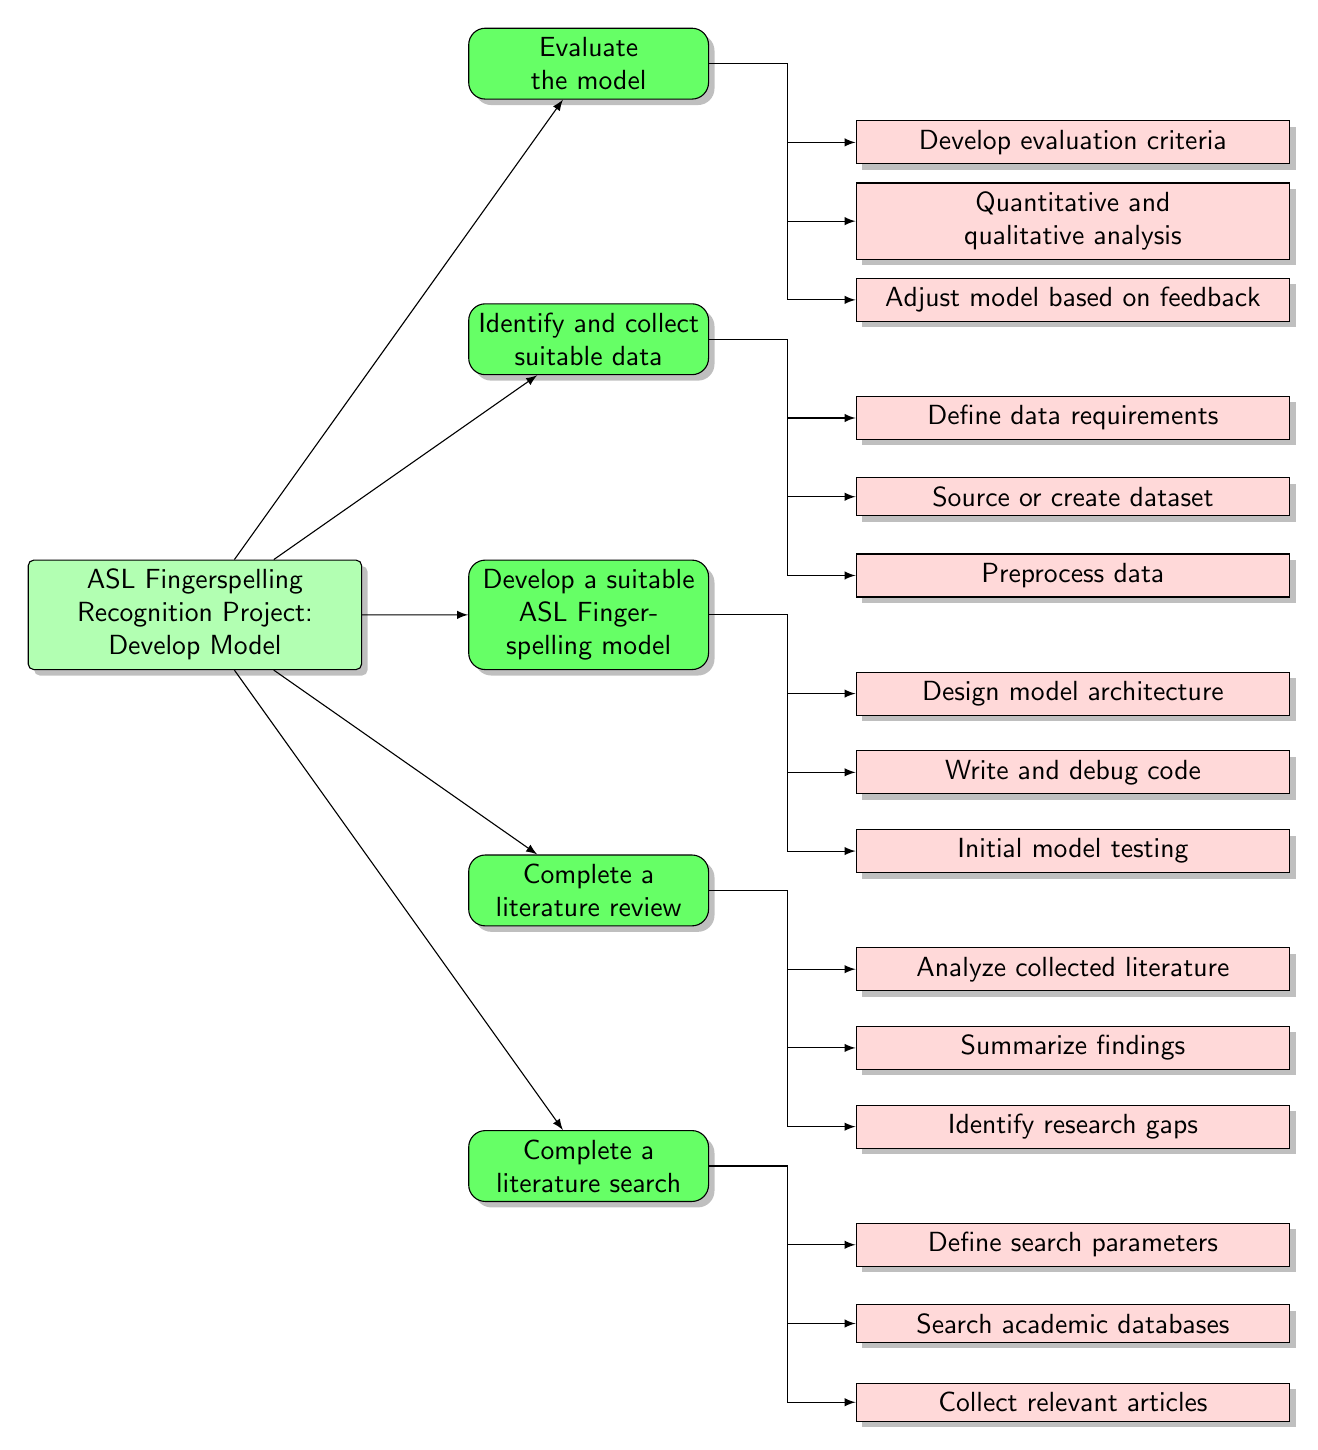
\begin{tikzpicture}[
                grow=right,
                level 1/.style={sibling distance=35mm, level distance=50mm},
                level 2/.style={sibling distance=35mm, level distance=40mm},
                level 3/.style={sibling distance=35mm, level distance=40mm},
                edge from parent/.style={->,draw},
                >=latex]
        \tikzset{
                basic/.style  = {draw, text width=4cm, drop shadow, font=\sffamily, rectangle},
                root/.style   = {basic, rounded corners=2pt, thin, align=center,
                                fill=green!30},
                level 2/.style = {basic, rounded corners=6pt, thin,align=center, fill=green!60,
                                text width=8em},
                level 3/.style = {basic, thin, align=center, fill=pink!60, text width=15em}
        }
        % root of the the initial tree, level 1
        \node[root] {ASL Fingerspelling Recognition Project: Develop Model}
        % The first level, as children of the initial tree
        child {node[level 2] (c1) {Complete a literature search}}
        child {node[level 2] (c2) {Complete a literature review}}
        child {node[level 2] (c3) {Develop a suitable ASL Fingerspelling model}}
        child {node[level 2] (c4) {Identify and collect suitable data}}
        child {node[level 2] (c5) {Evaluate the model}};

        % The second level, relatively positioned nodes
        \begin{scope}[every node/.style={level 3}]
                % Tasks for Complete a literature search
                \node [below of = c1, xshift=175pt] (c11) {Define search parameters};
                \node [below of = c11] (c12) {Search academic databases};
                \node [below of = c12] (c13) {Collect relevant articles};

                % Tasks for Complete a literature review
                \node [below of = c2, xshift=175pt] (c21) {Analyze collected literature};
                \node [below of = c21] (c22) {Summarize findings};
                \node [below of = c22] (c23) {Identify research gaps};

                % Tasks for Develop a suitable ASL Fingerspelling model
                \node [below of = c3, xshift=175pt] (c31) {Design model architecture};
                \node [below of = c31] (c32) {Write and debug code};
                \node [below of = c32] (c33) {Initial model testing};

                % Tasks for Identify and collect suitable data
                \node [below of = c4, xshift=175pt] (c41) {Define data requirements};
                \node [below of = c41] (c42) {Source or create dataset};
                \node [below of = c42] (c43) {Preprocess data};

                % Tasks for Evaluate the model
                \node [below of = c5, xshift=175pt] (c51) {Develop evaluation criteria};
                \node [below of = c51] (c52) {Quantitative and qualitative analysis};
                \node [below of = c52] (c53) {Adjust model based on feedback};
        \end{scope}

        % lines from each level 1 node to every one of its "children"
        % Continuous lines for each node without an arrow at the fork
        \foreach \parent in {1,...,5} {
                        % Draw a line to the fork point without an arrow
                        \path (c\parent.east) -- +(10mm,0) coordinate (fork\parent);
                        \draw (c\parent.east) -- (fork\parent);

                        % Create branches from the fork to each child with an arrow
                        \foreach \value in {1,2,3} {
                                        \draw[->] (fork\parent) |- (c\parent\value.west);
                                }
                };


\end{tikzpicture}



    \caption{Work Breakdown Structure: Develop Model}
    \label{fig:WBS: Develop Model}
\end{figure}
\newpage
\begin{landscape}
    \begin{figure}[h]
        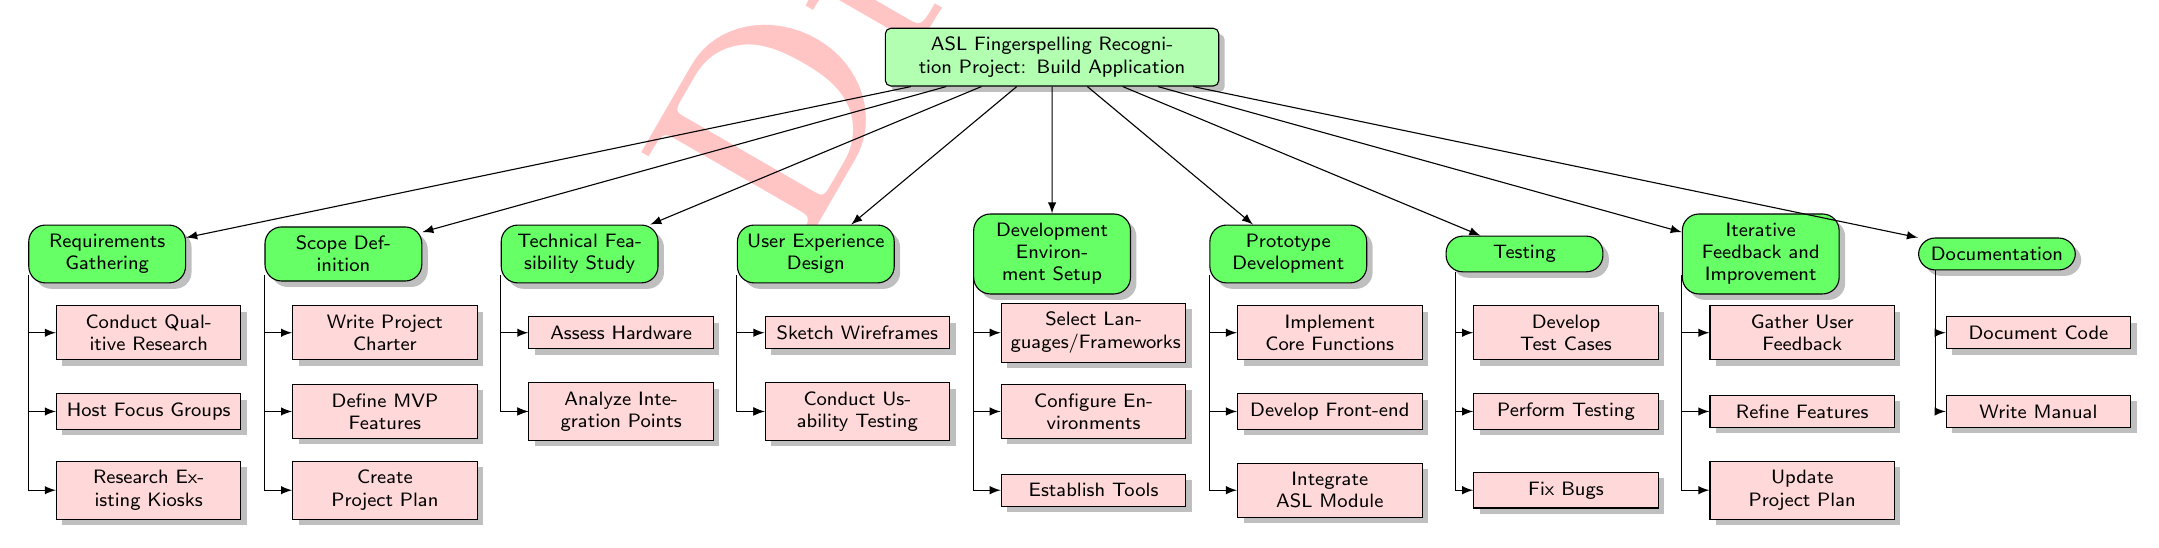
\begin{tikzpicture}[
                level 1/.style={sibling distance=30mm, level distance=25mm},
                level 2/.style={sibling distance=15mm},
                level 3/.style={sibling distance=15mm},
                edge from parent/.style={->,draw},
                >=latex]
        \tikzset{
                basic/.style  = {draw, text width=4cm, drop shadow, font=\sffamily\scriptsize, rectangle},
                root/.style   = {basic, rounded corners=2pt, thin, align=center,
                                fill=green!30},
                level 2/.style = {basic, rounded corners=6pt, thin,align=center, fill=green!60,
                                text width=5em},
                level 3/.style = {basic, thin, align=center, fill=pink!60, text width=6em}
        }
        % root of the the initial tree, level 1
        \node[root] {ASL Fingerspelling Recognition Project: Build Application}
        % The first level, as children of the initial tree
        child {node[level 2] (c1) {Requirements Gathering}}
        child {node[level 2] (c2) {Scope Definition}}
        child {node[level 2] (c3) {Technical Feasibility Study}}
        child {node[level 2] (c4) {User Experience Design}}
        child {node[level 2] (c5) {Development Environment Setup}}
        child {node[level 2] (c6) {Prototype Development}}
        child {node[level 2] (c7) {Testing}}
        child {node[level 2] (c8) {Iterative Feedback and Improvement}}
        child {node[level 2] (c9) {Documentation}};

        % The second level, relatively positioned nodes
        \begin{scope}[every node/.style={level 3}]
                % Tasks for Requirements Gathering
                \node [below of = c1, xshift=15pt] (c11) {Conduct Qualitive Research};
                \node [below of = c11] (c12) {Host Focus Groups};
                \node [below of = c12] (c13) {Research Existing Kiosks};

                % Tasks for Scope Definition
                \node [below of = c2, xshift=15pt] (c21) {Write Project Charter};
                \node [below of = c21] (c22) {Define MVP Features};
                \node [below of = c22] (c23) {Create Project Plan};

                % Tasks for Technical Feasibility Study
                \node [below of = c3, xshift=15pt] (c31) {Assess Hardware};
                \node [below of = c31] (c32) {Analyze Integration Points};

                % Tasks for User Experience Design
                \node [below of = c4, xshift=15pt] (c41) {Sketch Wireframes};
                \node [below of = c41] (c42) {Conduct Usability Testing};

                % Tasks for Development Environment Setup
                \node [below of = c5, xshift=15pt] (c51) {Select Languages/Frameworks};
                \node [below of = c51] (c52) {Configure Environments};
                \node [below of = c52] (c53) {Establish Tools};

                % Tasks for Prototype Development
                \node [below of = c6, xshift=15pt] (c61) {Implement Core Functions};
                \node [below of = c61] (c62) {Develop Front-end};
                \node [below of = c62] (c63) {Integrate ASL Module};

                % Tasks for Testing
                \node [below of = c7, xshift=15pt] (c71) {Develop Test Cases};
                \node [below of = c71] (c72) {Perform Testing};
                \node [below of = c72] (c73) {Fix Bugs};
                % Tasks for Iterative Feedback and Improvement
                \node [below of = c8, xshift=15pt] (c81) {Gather User Feedback};
                \node [below of = c81] (c82) {Refine Features};
                \node [below of = c82] (c83) {Update Project Plan};

                % Tasks for Documentation
                \node [below of = c9, xshift=15pt] (c91) {Document Code};
                \node [below of = c91] (c92) {Write Manual};
        \end{scope}

        % lines from each level 1 node to every one of its "children"
        % Loop over each parent
        % Loop over each parent
        \foreach \parent in {1,...,9} {
                        % Draw lines to child nodes that have been defined
                        \draw[->] (c\parent.195) |- (c\parent1.west);
                        \draw[->] (c\parent.195) |- (c\parent2.west);
                        % Check for exceptions with different number of children
                        \ifnum\parent=9
                                % Parent 9 only has 2 children
                        \else
                                \ifnum\parent=4
                                        % Parent 4 has 4 children
                                        \draw[->] (c\parent.195) |- (c\parent2.west);
                                \else
                                        \ifnum\parent=3
                                                % Parent 3 has 4 children
                                                \draw[->] (c\parent.195) |- (c\parent2.west);
                                        \else
                                                % All other parents have 3 children
                                                \draw[->] (c\parent.195) |- (c\parent3.west);
                                        \fi
                                \fi
                        \fi
                }
\end{tikzpicture}

        \caption{Work Breakdown Structure: Build Application}
        \label{fig:WBS: Build Application}
    \end{figure}
\end{landscape}
\newpage
\begin{figure}[h]
    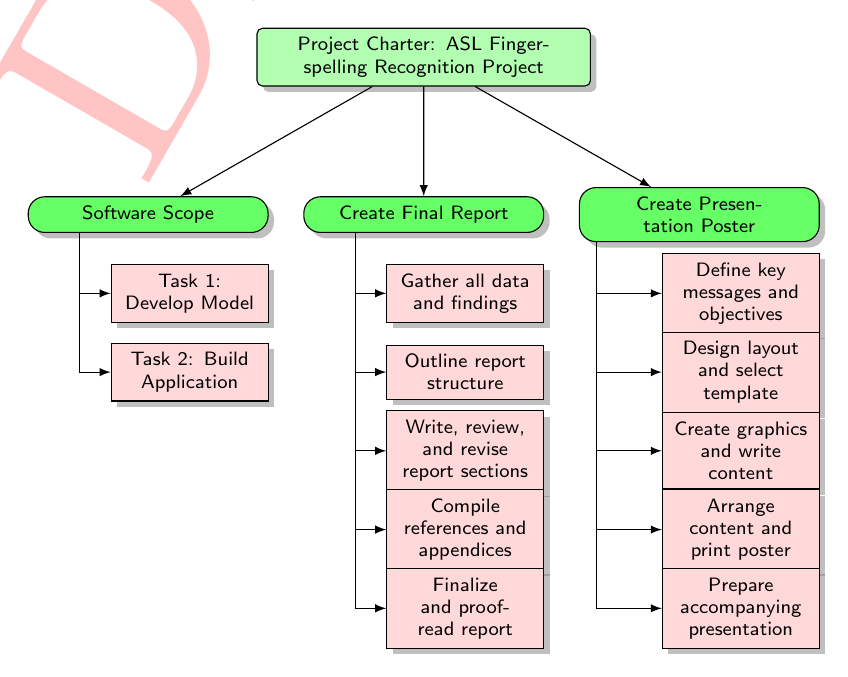
\begin{tikzpicture}[
                level 1/.style={sibling distance=35mm, level distance=20mm},
                level 2/.style={sibling distance=25mm, level distance=20mm},
                level 3/.style={sibling distance=35mm, level distance=20mm},
                edge from parent/.style={->,draw},
                >=latex]
        \tikzset{
                basic/.style  = {draw, text width=4cm, drop shadow, font=\sffamily\scriptsize, rectangle},
                root/.style   = {basic, rounded corners=2pt, thin, align=center,
                                fill=green!30},
                level 2/.style = {basic, rounded corners=6pt, thin,align=center, fill=green!60,
                                text width=8em},
                level 3/.style = {basic, thin, align=center, fill=pink!60, text width=5em}
        }
        % root of the the initial tree, level 1
        \node[root] {Project Charter: ASL Fingerspelling Recognition Project}
        % The first level, as children of the initial tree
        child {node[level 2] (c1) {Software Scope}}
        child {node[level 2] (c3) {Create Final Report}}
        child {node[level 2] (c4) {Create Presentation Poster}};

        % The second level, relatively positioned nodes
        \begin{scope}[every node/.style={level 3}]
                % Tasks for Complete a literature search
                \node [below of = c1, xshift=15pt] (c11) {Task 1: Develop Model};
                \node [below of = c11] (c12) {Task 2: Build Application};

                % Tasks for Create Final Report
                \node [below of = c3, xshift=15pt] (c31) {Gather all data and findings};
                \node [below of = c31] (c32) {Outline report structure};
                \node [below of = c32] (c33) {Write, review, and revise report sections};
                \node [below of = c33] (c34) {Compile references and appendices};
                \node [below of = c34] (c35) {Finalize and proofread report};

                % Tasks for Create Presentation Poster
                \node [below of = c4, xshift=15pt] (c41) {Define key messages and objectives};
                \node [below of = c41] (c42) {Design layout and select template};
                \node [below of = c42] (c43) {Create graphics and write content};
                \node [below of = c43] (c44) {Arrange content and print poster};
                \node [below of = c44] (c45) {Prepare accompanying presentation};
        \end{scope}

        % lines from each level 1 node to every one of its "children"
        % Continuous lines for each node without an arrow at the fork

        \foreach \value in {1,2}
        \draw[->] (c1.195) |- (c1\value.west);

        \foreach \value in {1,...,5}
        \draw[->] (c3.195) |- (c3\value.west);

        \foreach \value in {1,...,5}
        \draw[->] (c4.195) |- (c4\value.west);

\end{tikzpicture}



    \caption{Work Breakdown Structure}
    \label{fig:WBS: Project Charter}
\end{figure}
\newpage
\begin{landscape}
    \begin{figure}[h]
        \centering
        % Placeholder for the Gantt chart
        \fbox{\parbox{15cm}{\centering Gantt chart placeholder \\ (Refer to the accompanying zipped file for the full chart)}}
        \caption{Gantt Chart}
        \label{fig:GanttChart}
    \end{figure}
    In this report's accompanying zipped file, a detailed Gantt chart is included as a separate document. Due to its extensive size and complexity, it is provided as an individual file to facilitate detailed review and ensure clarity. Please refer to the zipped file named gantt-project.png for the complete Gantt chart, which offers an in-depth view of the project timeline and milestones.
\end{landscape}
\begin{figure}[h]
    \begin{longtable}{|>{\raggedright\arraybackslash}p{3cm}|>{\raggedright\arraybackslash}p{3cm}|>{\raggedright\arraybackslash}p{2cm}|>{\raggedright\arraybackslash}p{2cm}|>{\raggedright\arraybackslash}p{3cm}|}
    \hline
    \textbf{Risk} & \textbf{Impact} & \textbf{Probability} & \textbf{Status} & \textbf{Mitigation Strategy} \\
    \hline
    \endhead
    % Risks here...
    Inaccurate ASL Recognition & High & Medium & Open & Enhance data collection and improve algorithm accuracy. \\
    \hline
    Data Privacy Concerns & High & High & Open & Implement GDPR compliant data handling processes. \\
    \hline
    Loss of Data & High & Low & Open & Implement GoogleDrive and GitHub repository. \\
    \hline
    Loss of Project Supervisor & High & Low & Open & Maintain regular communication with supervisor. \\
    \hline
    Project Delays & Medium & High & Open & Develop a schedule with buffers and regularly update it. \\
    \hline
    User Adoption Challenges & Medium & High & Open & Engage with users early and incorporate feedback. \\
    \hline
    Technology Integration Issues & Medium & Medium & Open & Conduct compatibility testing. \\
    \hline
\end{longtable}
    \caption{Risk register}
    \label{fig:Risk Register}
\end{figure}
\newpage
\section{Meetings With Supervisor} \label{K}
\pagenumbering{arabic} % Reset page numbering
\renewcommand{\thepage}{K\arabic{page}}
\newpage
\begin{longtable}{|p{2cm}|p{2cm}|p{3cm}|p{4cm}|p{4cm}|}
    \hline
    \textbf{Date}    & \textbf{Time} & \textbf{Location} & \textbf{Purpose}                        & \textbf{Description and Actions}                                                                                                                                                   \\
    \hline
    \endhead
    15 November 2023 & 13:00 – 14:00 & CCCU - Lg33       & Discuss project and literature research & Reviewed current status, discussed challenges, and agreed on next steps including further research on ASL recognition and user-centric approach to requirements. Contact charities \\
    \hline
    29 November 2023 & 13:00 - 14:00 & CCCU - Lg33       & ?                                       & ?                                                                                                                                                                                  \\
    \hline
\end{longtable}
\section{Agile Development: Timebox 1}
\pagenumbering{arabic} % Reset page numbering
\renewcommand{\thepage}{L\arabic{page}}
\newpage
Not applicable.
\section{Agile Development: Timebox 2}
\pagenumbering{arabic} % Reset page numbering
\renewcommand{\thepage}{M\arabic{page}}
\newpage
Not applicable.
\section{Agile Development: Timebox 3}
\pagenumbering{arabic} % Reset page numbering
\renewcommand{\thepage}{N\arabic{page}}
\newpage
Not applicable.

\end{document}